\chapter{ShEx-Lite Demo Paper}\label{ap:shex-lite-paper}
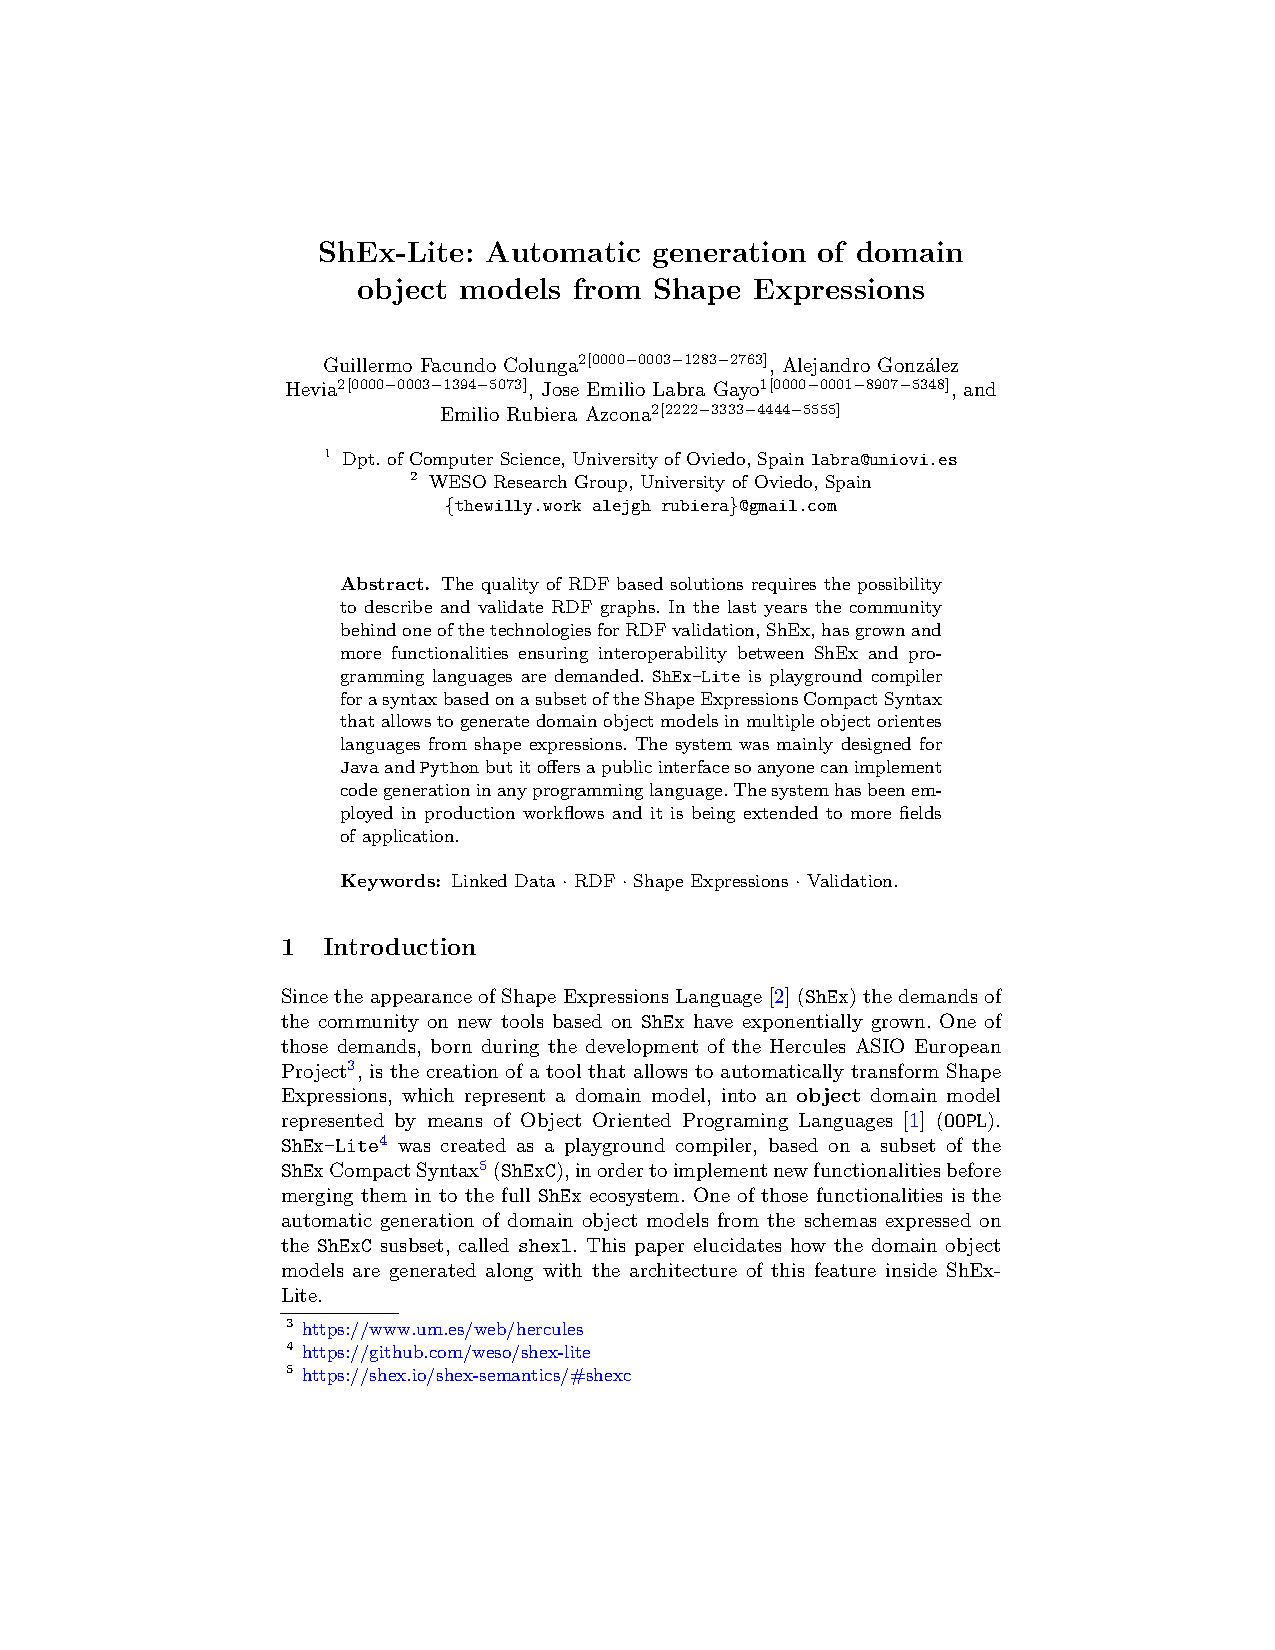
\includepdf[pages=-]{images/shex-lite-demo-paper.pdf}

\begin{figure}
    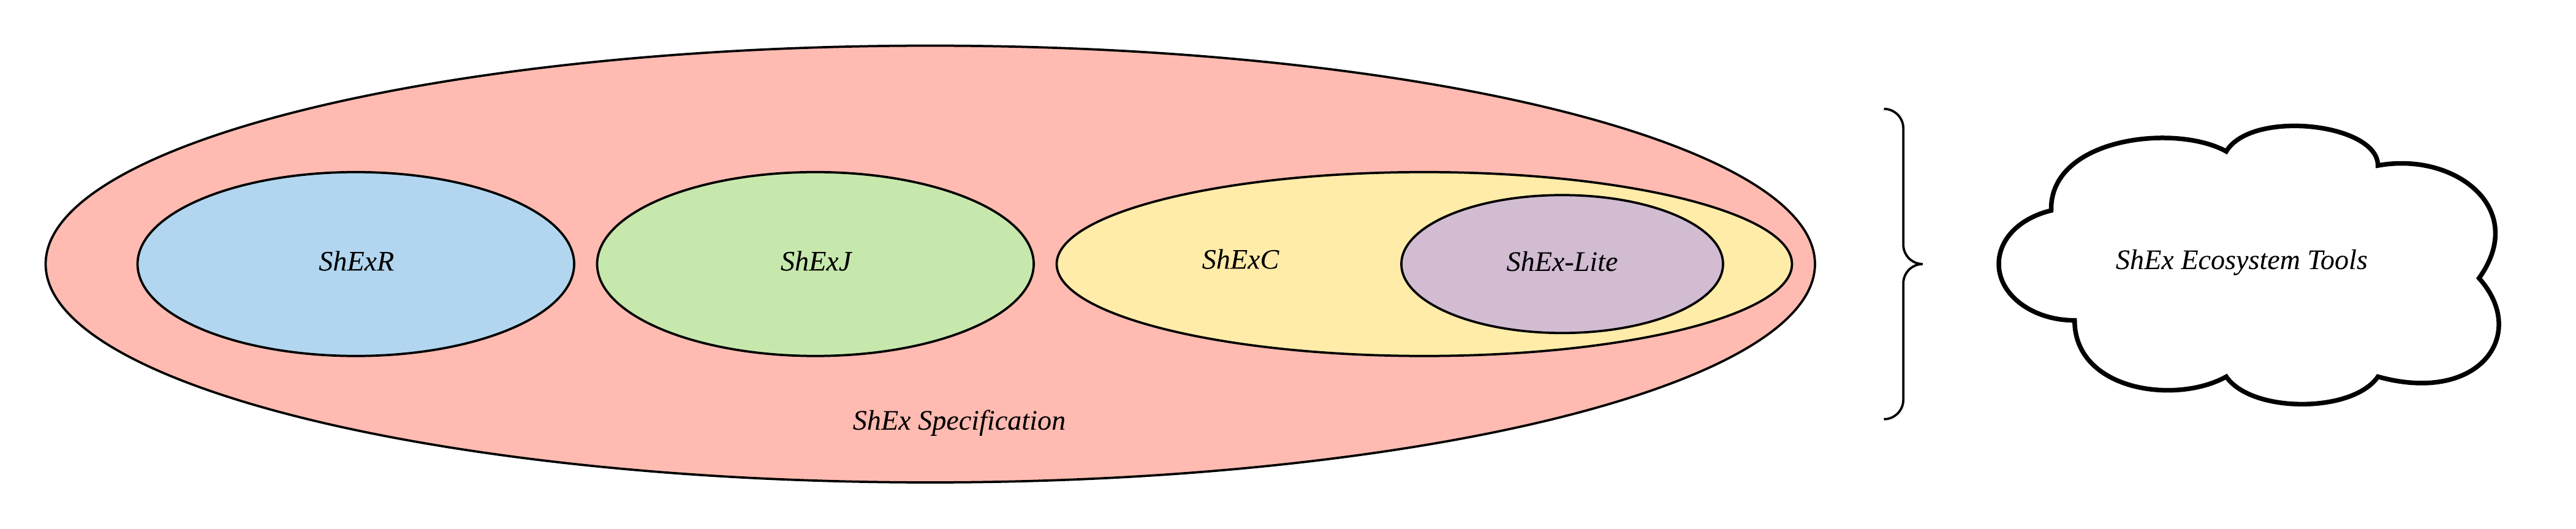
\includegraphics[width=\textwidth]{images/shex-lite-syntaxes-mental-model.png}
    \centering
    \caption[Mental model of ShEx-Lite in the existing ShEx syntaxes context.]{Mental model of
    ShEx-Lite in the existing ShEx syntaxes context. From this model we can see that Shex-Lite
    is in fact an strictly subset of ShExC, which follows the ShEx Specification. And therefore
    ShEx-Lite will also follow that expecification, which automatically enables ShEx-Lite schemas
    to be used in any other existing ShEx tool.}
    \label{fig:syntax-mental-model}
\end{figure}

\begin{figure}
  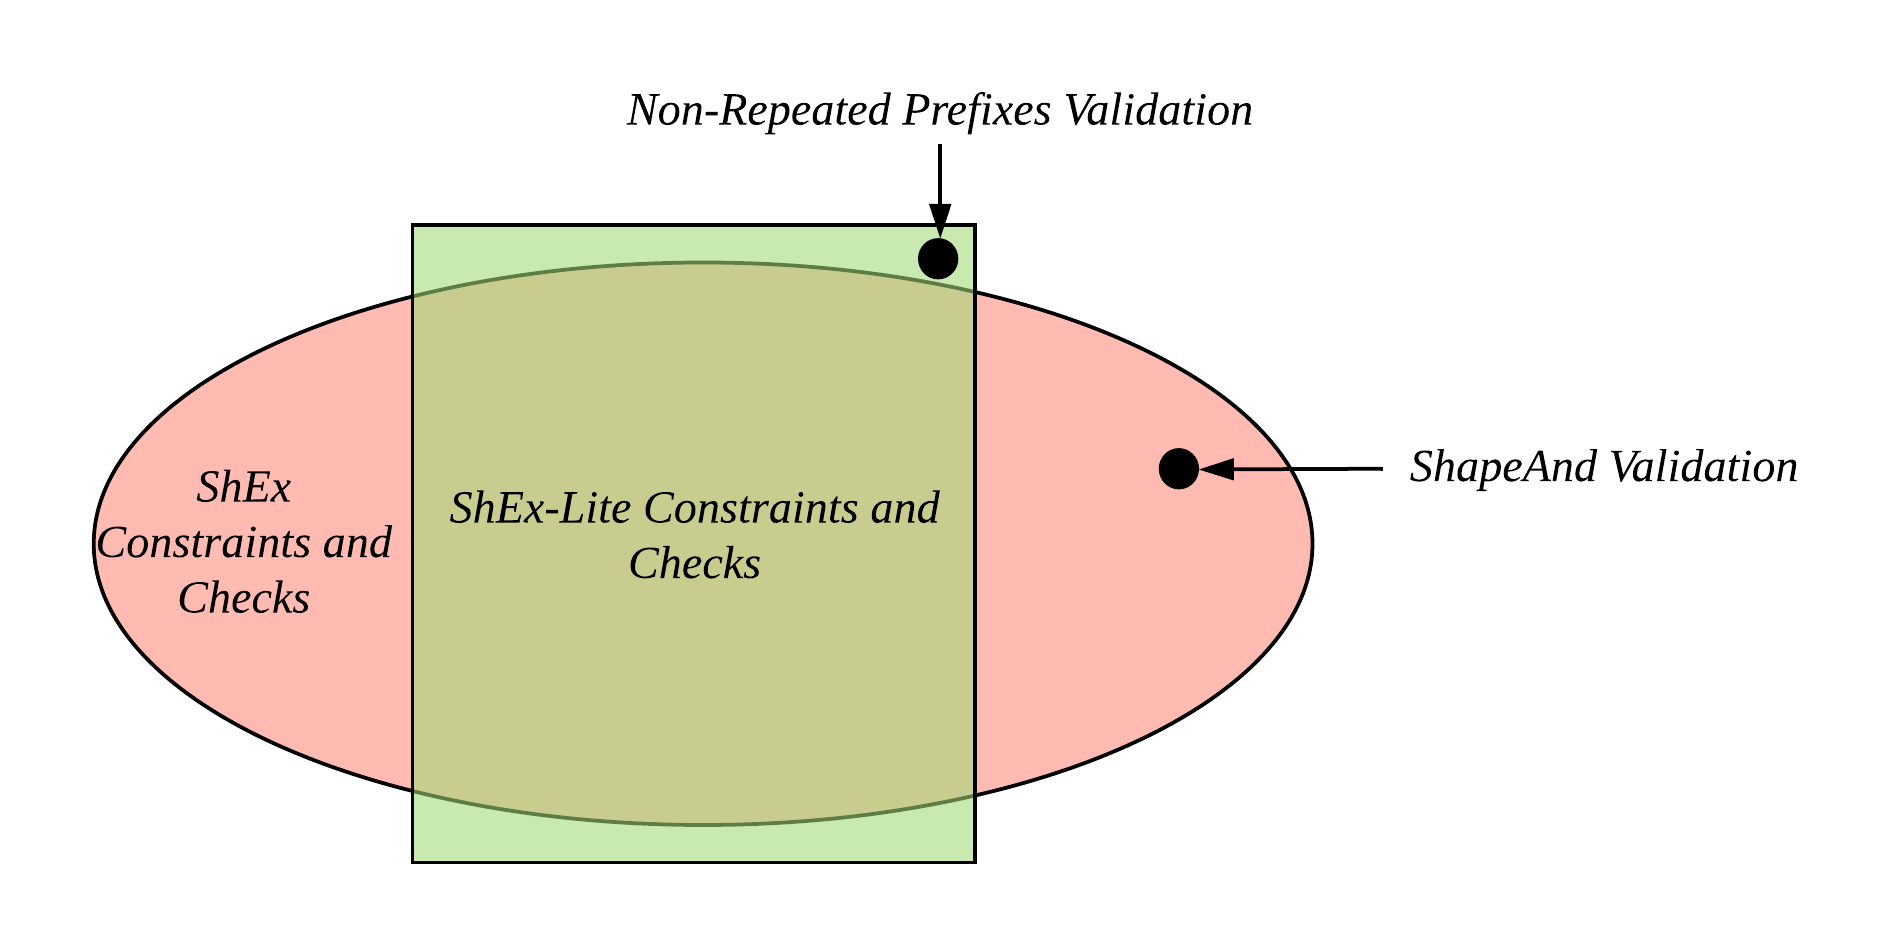
\includegraphics[width=\textwidth]{images/shex-lite-constraints-context.png}
  \centering
  \caption[Constraints and checks context diagram for ShEx-Lite and ShEx.]{Constraints
  and checks context diagram for ShEx-Lite and ShEx.}
  \label{fig:constraints-context}
\end{figure}